\documentclass[a4paper,10pt]{report}

\topmargin -2cm
%\topskip0cm
%\footskip0cm
%\headsep0cm
\parindent0cm
\oddsidemargin -1cm
\evensidemargin -1cm
\headheight 2cm
\textheight 24cm
\textwidth 18cm

\author{Daniel W\"aber (4049590)}
\title{\"Ubung}

\usepackage{ucs}
\usepackage[utf8x]{inputenc}
\usepackage{german}
\usepackage{color}
\usepackage{url}
\usepackage{graphicx}
\usepackage{algorithmic}

\pagestyle{empty}
\usepackage{makeidx}
\usepackage{amsmath}
\usepackage{amsfonts}
\usepackage{amssymb,euscript}
\usepackage{dsfont}
\usepackage{listings}
\usepackage{enumerate}
\newfont{\Fr}{eufm10}
\newfont{\Sc}{eusm10}
\newfont{\Bb}{msbm10}
\newcommand{\limin}{\lim_{n\rightarrow\infty}}
\newcommand{\limix}{\lim_{x\rightarrow\infty}}
\newcommand{\limun}{\lim_{n\rightarrow -\infty}}
\newcommand{\limux}{\lim_{n\rightarrow -\infty}}
\newcommand{\limx}{\lim_{x\rightarrow x_0}}
\newcommand{\limh}{\lim_{h\rightarrow 0}}
\newcommand{\defi}{\paragraph{Definition:}}
\newcommand{\bew}{\paragraph{Beweis:}}
\newcommand{\satz}{\paragraph{Satz:}}
\newcommand{\bsp}{\paragraph{Beispiel:}}
\newcommand{\lemma}{\paragraph{Lemma:}}
\newcommand{\N}{\mathds{N}}
\newcommand{\F}{\mathds{F}}
\newcommand{\Z}{\mathds{Z}}
\newcommand{\Q}{\mathds{Q}}
\newcommand{\R}{\mathds{R}}
\newcommand{\G}{\mathds{G}}
\newcommand{\C}{\mathds{C}}
\newcommand{\K}{\mathds{K}}
\newcommand{\A}{\mathds{A}}
\newcommand{\E}{\mathcal{E}}
\renewcommand{\P}{\mathcal{P}}
\newcommand{\sigA}{$\sigma$-Algebra }
\newcommand{\qed}{$\hfill\blacksquare$}
\newcommand{\arsinh}{\operatorname{arsinh} }
\newcommand{\arcosh}{\operatorname{arcosh} }
\newcommand{\gdw}{ $ \Leftrightarrow $ }
\newcommand{\tf}{ $ \Rightarrow $ }
\newcommand{\mgdw}{\Leftrightarrow}
\newcommand{\mtf}{\Rightarrow}
\newcommand{\Bild}{\text{Bild}}
\newcommand{\Kern}{\text{kern}}
\newcommand{\rg}{\text{rg}}
\newcommand{\deff}{\text{deff}}

\newcommand{\alphato}{\underset{\alpha}\to}
\newcommand{\betato}{\underset{\beta}\to}
\newcommand{\etato}{\underset{\eta}\to}
\newcommand{\ito}{\underset{i}\to}
\newcommand{\sto}{\underset{s}\to}
\newcommand{\kto}{\underset{k}\to}
\newcommand{\xto}{\underset{x}\to}

\usepackage{fancyhdr}
\pagestyle{fancy}
\lhead{Daniel Waeber\\Alex Muenn}
\chead{"Ubungsblatt \nr\\\today}
\rhead{Bildverarbeitung}


\newcommand{\nr}{6}
\lstset{language=matlab}

\begin{document}
\section*{Aufgabe 1 - Histogram}
\paragraph{Berechnung des Histogramms}
In einem Array der Groesse der Graustufen werden die Pixel des zugehehoerigen
Wertes im Bild gezaehlt und anschliessend wird das Histogramm normalisiert.

\begin{figure}[H]
\begin{center}
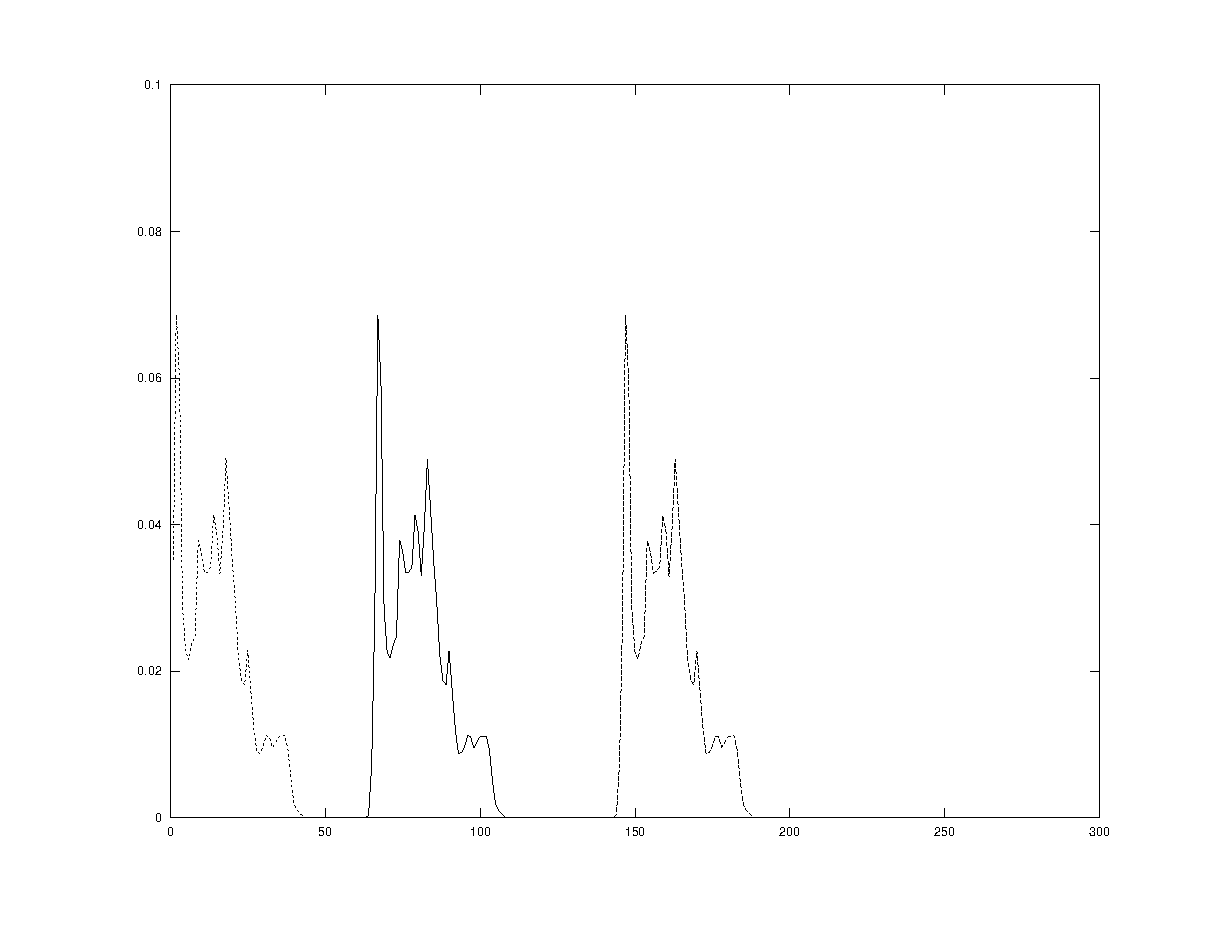
\includegraphics[width=100mm]{u06/task1-hist.eps}
\end{center}
\caption{Histogramme der Lena-Bilder}
\end{figure}

\paragraph{Angleichung}
Mit Hilfe der cumsum function kann die Verteilungsfunction berechnent werden.

Anschliessend kann auf jedes Pixel die in der Vorlesung vorgestellte Normailsierungsfunction angewandt werden:
\begin{equation}
y = \frac{cdf(x) - m}{1 - m}
\end{equation}
wobei $m$ den ersten Wert im Histogram der ungleich 0 ist darstellt.

\begin{figure}[H]
\begin{center}
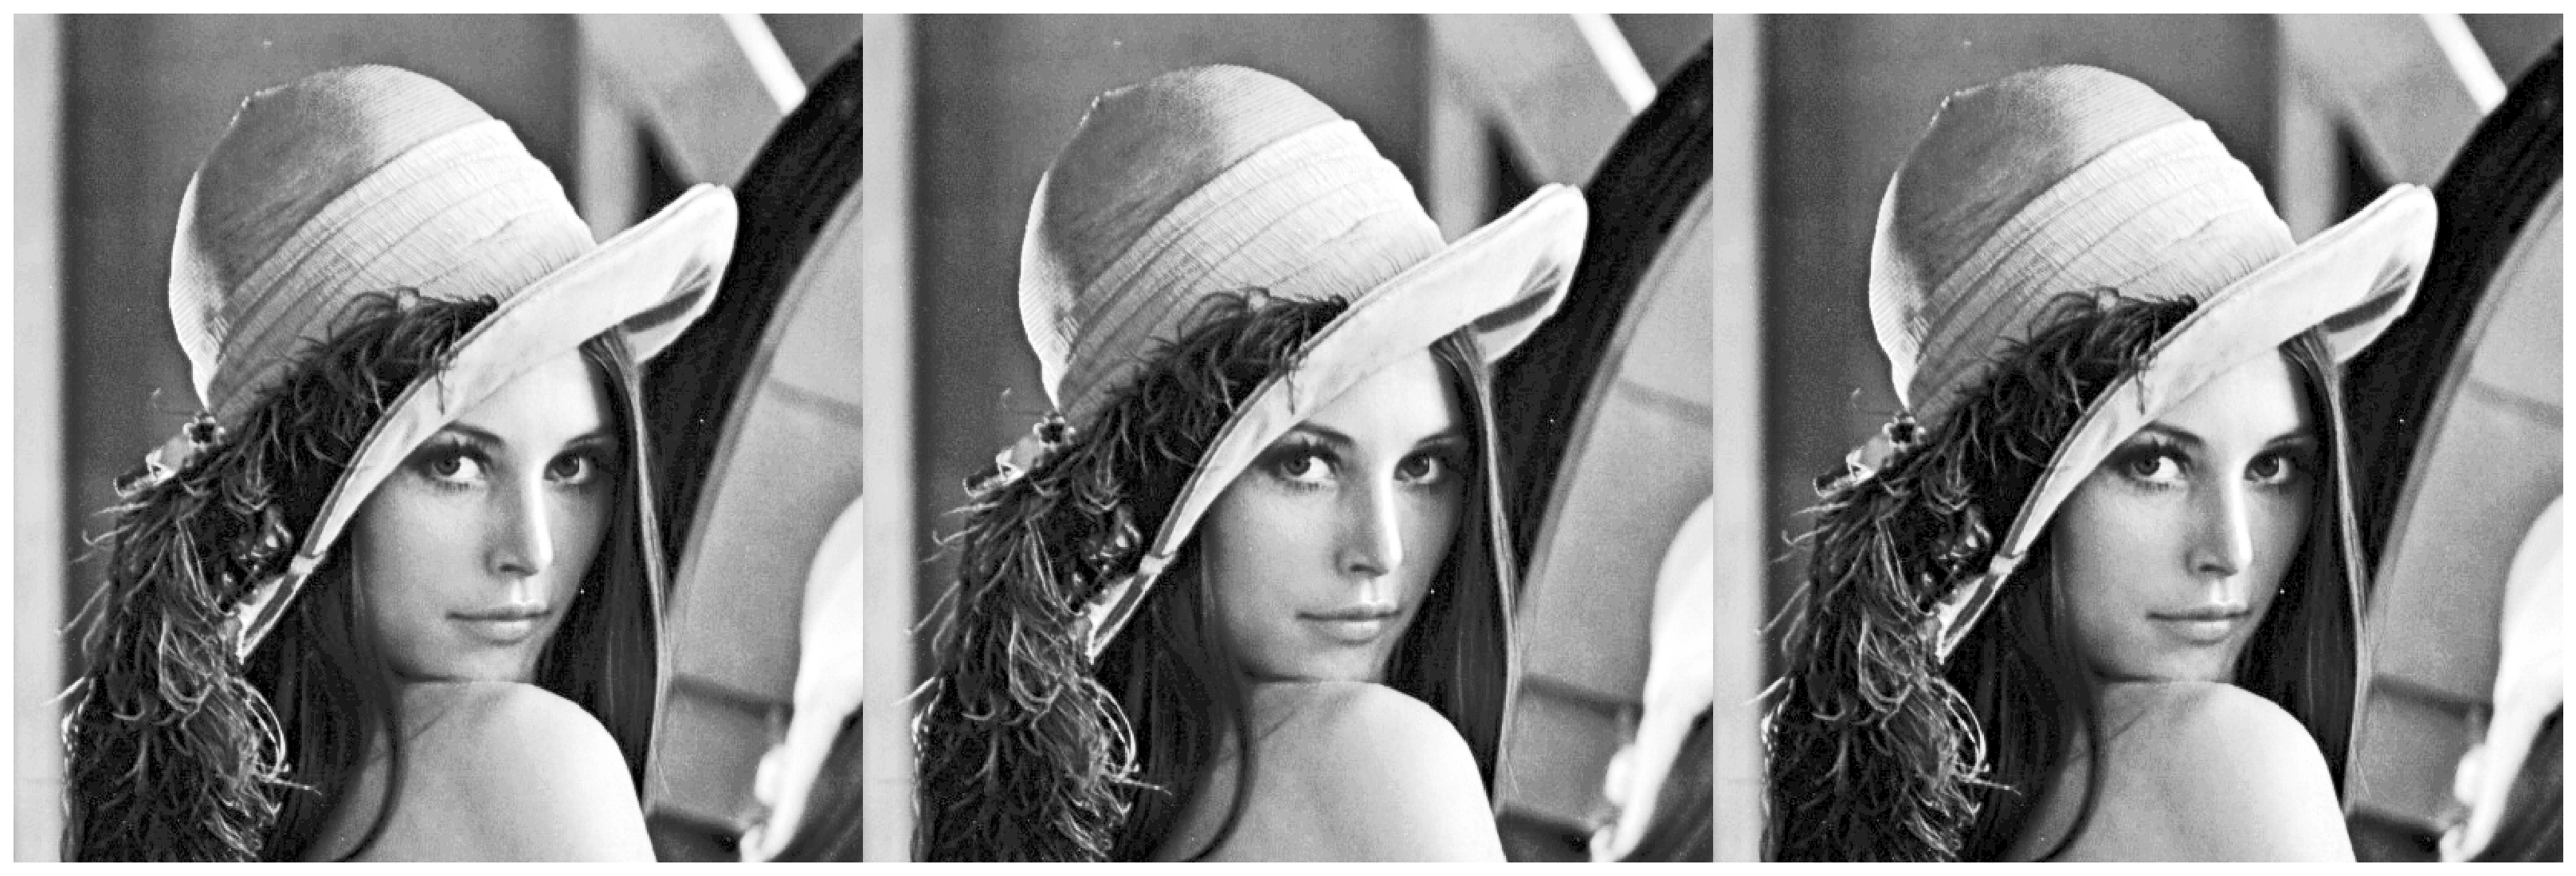
\includegraphics[width=150mm]{u06/task1-eq.eps}
\end{center}
\caption{Ergebniss der Angleichung}
\end{figure}

\section*{Aufgabe 2 - Kantenerkennung}
\paragraph{Noise Reduction}
Anwendung eines Gausfilters mit $\sigma=1$ wie in Aufgabe 3 fuhrt zur Veringerung des Rauschens.

\paragraph{Derivative}
Die Ableitung in $x$ bzw. $y$ kann auch wie in Aufgabe 3 mit Hilfe des Sobel-Filters bestimmt werden.

\paragraph{Non-maxima Supression}
Die Umrechnung in Polar-Koordinaten erfolgt mit \lstinline@card2pol(Ix, Iy)@.

Anschliessend wird der Winckel auf 0, 45, 90 und 135 normalisiert und gerunden und anhand des
Winkels bestimmt, welche umliegenden Fehlder fuer einen Pixel zur NMS betrachtet werden muessen.
Ist die Groesse der Ableitung (Radius in Polar) bei einem Pixel nicht mximal in
den betrachteten Felder, wird dies auf 0 gesetzt.

\paragraph{Thresholding und Tracking}
Fuer alle Pixel, deren Ableitung groesser als \lstinline@maxtres@ ist, wird die Track-Function aufgerufen,
die rekursive alle Pixel in die Richtung der Kante deren Ableitung groesser als \lstinline@mintres@ ist,
makiert.

\begin{figure}[H]
\begin{center}
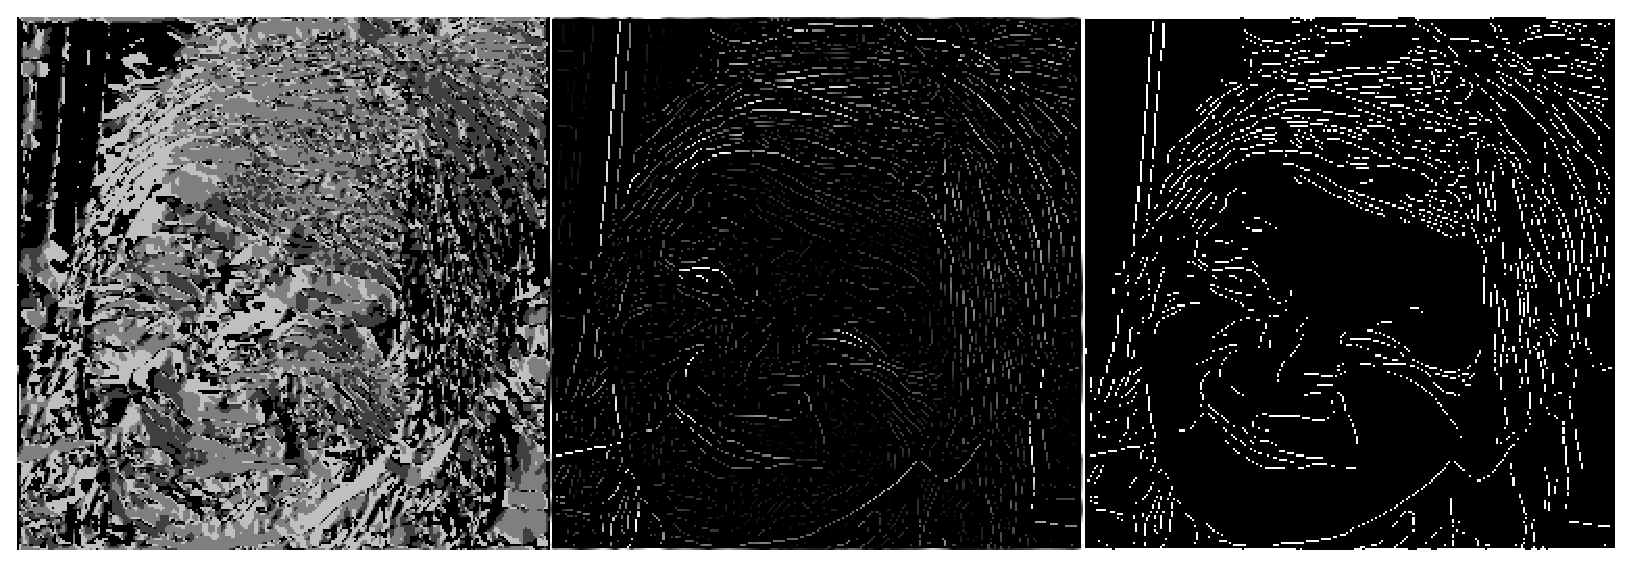
\includegraphics[width=150mm]{u06/t2.eps}
\end{center}
\caption{Kantenerkennung mit Zwischenschritten}
\end{figure}

\section*{Aufgabe 3 - Morphologische Operatoren}
\paragraph{Dilate und Erode}
Die Maske kann mit \lstinline@and@ bzw. \lstinline@or@ und  \lstinline@not@ auf Teilstucke des Bildes angewandt werden und anschliessend
wird der Wert des Pixels an der Stelle mit \lstinline@any@ bzw. \lstinline@all@ darauf bestimmt werden.

\begin{figure}[H]
\begin{center}
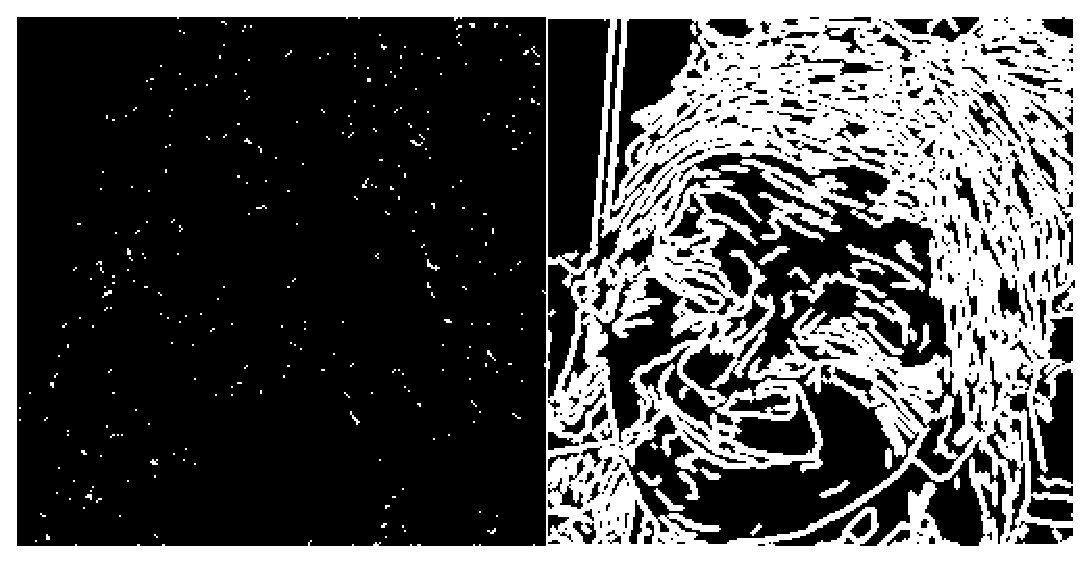
\includegraphics[width=100mm]{u06/t3-ed.eps}
\end{center}
\caption{Erode und Dilate}
\end{figure}

\paragraph{Close und Open}
Durch Verknuepfung von Dilate und Erode

\begin{figure}[H]
\begin{center}
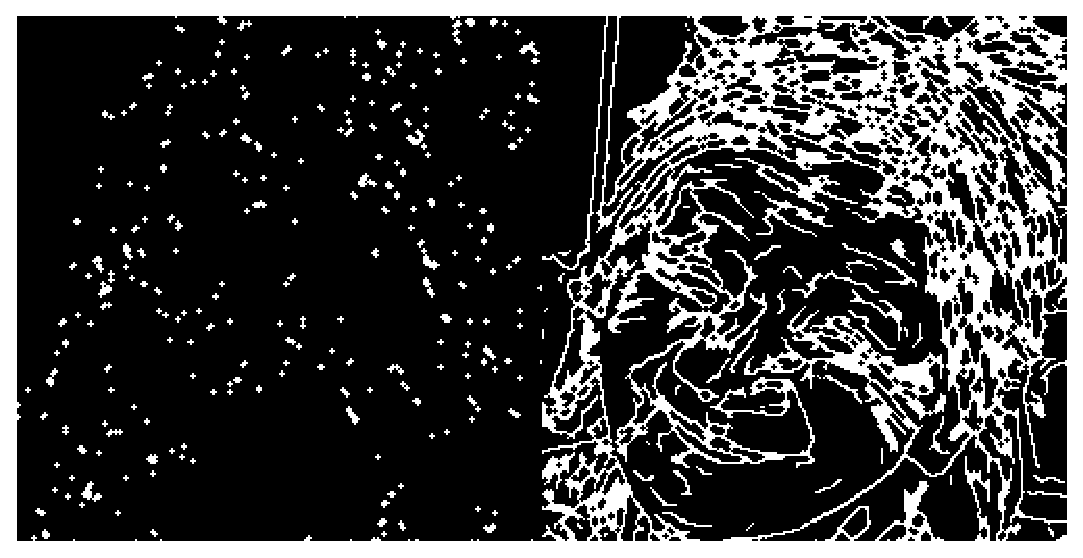
\includegraphics[width=100mm]{u06/t3-co.eps}
\end{center}
\caption{Open und Close}
\end{figure}

\end{document}
